%!TEX root = ../main.tex
%Motor data object: 4600h. includes motor slip frequency (not relevant), currents, voltages and temperature of heatsink. Don't know yet what the subindices are.
%It is possible to map them to Process Data Object for fixed time updates. It doesn't say anywhere what update rate, we can achieve.
%I've gotten a good amount of data from Karsten.

%This section assumes that CANOpen has been adequately explained beforehand

\subsection{Interfacing with Sevcon}\label{sub:Sevcon_interfacing}
The working motor driver currently on the go-kart is in fact compatible with CAN.
However, as it is a general purpose motor driver, it cannot be programmed to used the high level protocol designed in this project. 
For this reason, and to make the network unaffected by replacement of the motor driver, it has been decided to use a Zybo to interface with the Sevcon.

\subsubsection{Physical Connection}\label{sub:sevcon_physical_connection}~\\
Communication with the Sevcon is done through a high speed CAN bus that needs to adhere to ISO11898-2.
As described in section~\ref{sub:CANphys}, one transceiver board has two transceivers along with a terminal so that one Zybo can connect to the Sevcon using the second CAN controller.
It is recommended to use twisted pair wires with cross section area ranging from $0.5 \si{\milli \meter \squared}$ to $1.5 \si{\milli \meter \squared}$, and terminating the Zybo end with $120 \si{\ohm}$.
On the Sevcon, this can be done by shorting pins 2 and 24, to utilize an internal termination resistor.
There are two CAN interfaces: Pins 13(+) and 24(-) are used for configuration, and pins 16(+) and 27(-) are used to interface with other CAN devices.
The 35 pin connector is shown below for reference:

\begin{figure}[h]
	\centering
	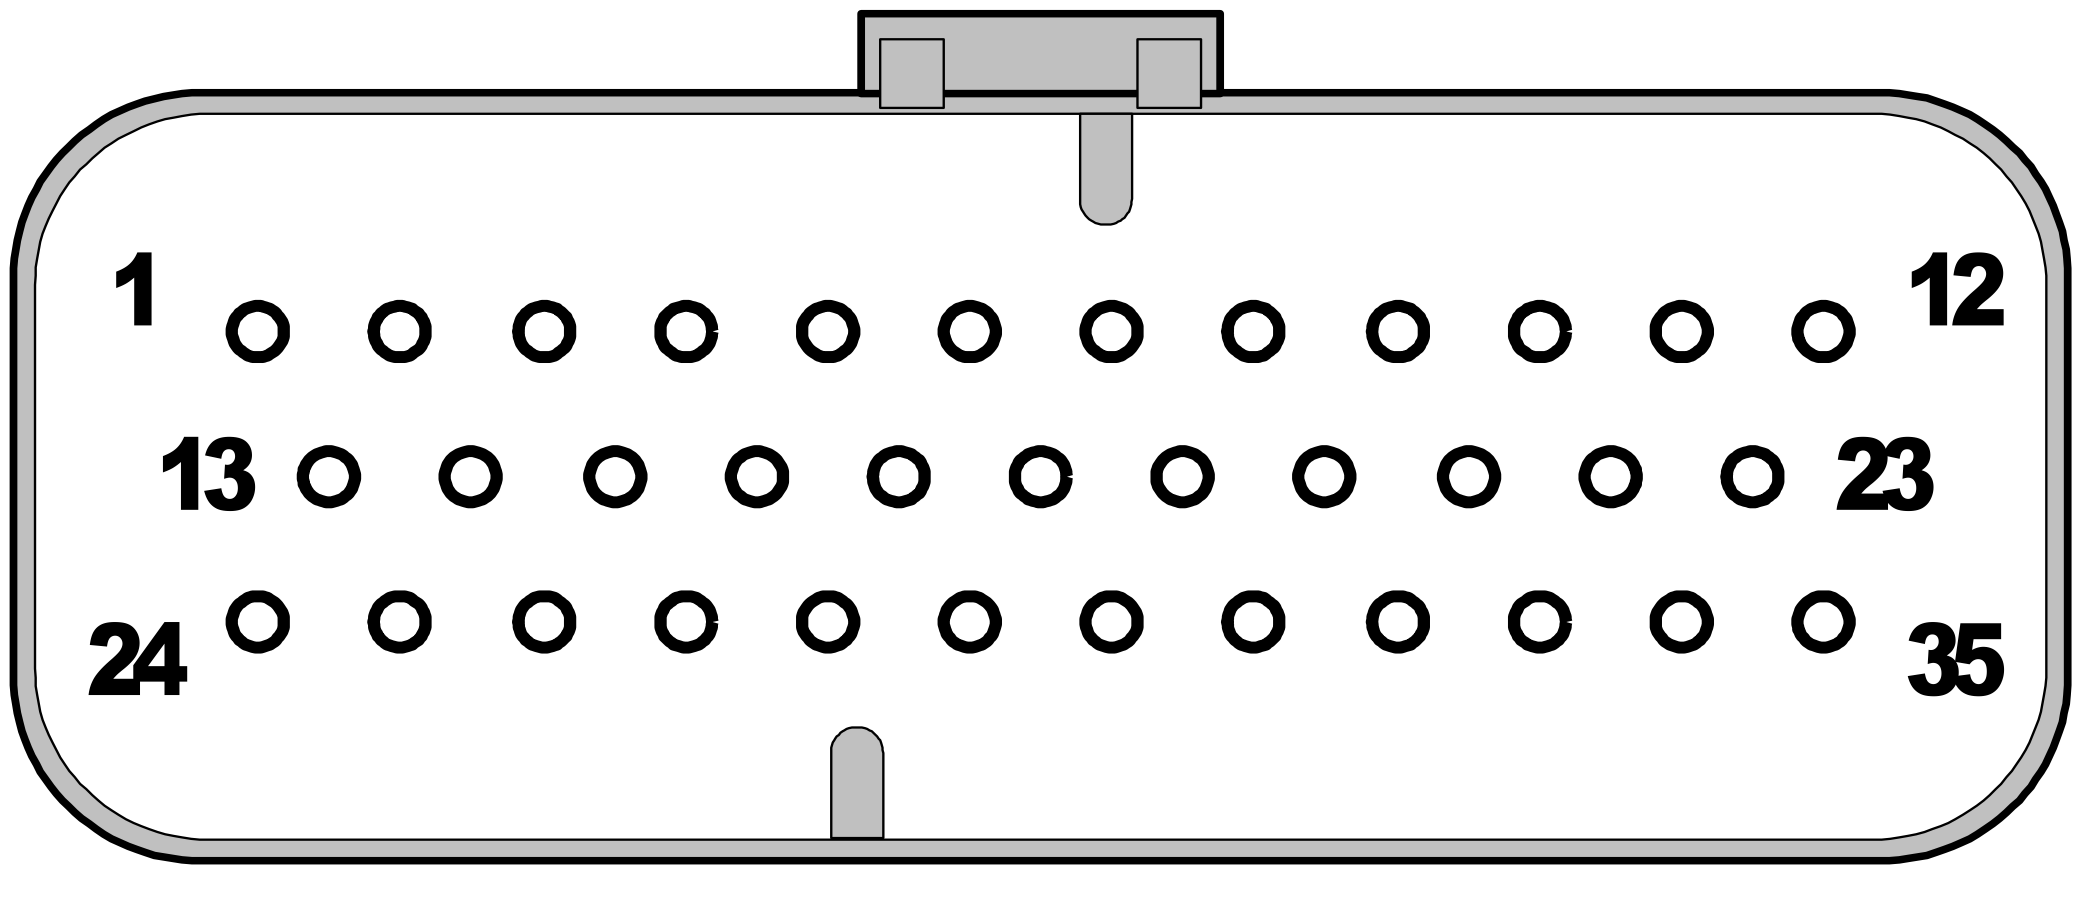
\includegraphics[width = 0.6\linewidth]{graphics/35_pin_dsub}
	\caption{The 35 pin AMPSeal connector used to interface with the Sevcon}
	\label{fig:35_pin_dsub}
\end{figure}

\subsubsection{Sevcon Object Dictionary}\label{sub:sevcon_object_dictionary}~\\
The Sevcon utilizes CAN open, which means all it's parameters are listed in an object dictionary.
Because the Sevcon is a general purpose AC motor driver, its object dictionary is very large, and holds a lot of objects that are completely irrelevant for this particular setup, such as motor slip, and speed control parameters. 
The object directory is documented in a 1400+ Excel file. 
Some objects of interest are:

\begin{table}[h]
	\centering
	\begin{tabular}{| c | c | c | c |}
		\hline
		Parameters & Index-subindex & Read/Write & Map to PDO \\ % Excel line
		\hline
		Measured Id & 4600h-7 & Read & Yes \\ %981
		Measured Iq & 4600h-8 & Read & Yes \\ %982
		Measured Vd & 4600h-9 & Read & Yes \\ %983
		Measured Vq & 4600h-10 & Read & Yes \\ %984
		Target Id & 4600h-5 & Read & Yes \\ %979
		Target Iq & 4600h-6 & Read & Yes \\ %980
		Encoder Read-out & 4630h-9 to -12 & Read & Yes \\ %1137
		Throttle value & 2620h & Read & Yes \\ %330
		Velocity & 606Ch & Read & Yes \\ %1378
		\hline	
	\end{tabular}
	\caption{List of some of the parameters readable and writeable through CANOpen}
	\label{tab:parameters_of_interest}
\end{table}

For the most part, these values in 16 bit resolution, which means they can be grouped together four at a time in a PDO.
The fact that a value can be mapped to PDO means, that it can be transmitted to the Zybo at fixed time intervals or whenever it is updated.
The Encoder Read-out sin/cosine encoder position, so it needs to be converted to mechanical angle. 
This is done using equation~\ref{eq:cos_sin_to_degree}

\begin{equation}
\Omega_m = \mathrm{atan2}(\cos,\sin)
\label{eq:cos_sin_to_degree}
\end{equation}

These adaptations need to be done to make the Sevcon node a generic motor driver node.
That way it would be possible to use this system with a custom made inverter.
